\documentclass[../master]{subfiles}

%\graphicspath{{../eps/}{../pic/}}

\begin{document}

\chapter{はじめに}
\section{宇宙での元素合成過程}
\label{seq::nucleaosynthesis}
身の回りには多種多様な物質が存在している。
これらの物質は原子が組み合わさることで形成される。
現在の地球には水素 (原子番号1) からウラン (原子番号92) までの元素が天然で存在してる。
原子は更に小さい原子核と電子で構成されており、原子核は陽子と中性子で構成されている。
現在までに天然、人工合わせて118種類の元素が確認されている。
しかし、ビッグバン直後には水素とヘリウムと僅かな軽元素しか存在していなかったと考えられている。
これは、質量数 (A) が5及び8の安定な原子核が存在しないことに由来する。
ヘリウム4 ($\alpha$) は安定な原子核である。
2つの$\alpha$が反応し${}^{8}{\rm Be}$が生成されても、
2つの$\alpha$に分裂するほうが安定であるためすぐに崩壊してしまう。
同様にA = 5の原子核が生成してもすぐに軽い核2つに分裂してしまう。

そのため、宇宙初期では水素を主成分とする恒星しか存在しなかったと考えられる。
このような恒星が重力により収縮し中心温度が$10^7~{\rm K}$を超えると、
陽子 (水素) が反応してより$\alpha$が合成されるppチェインによって水素の燃焼が行われるようになる。
ppチェインでは図\ref{fig::pp_chain}に示した3つの系列が重要とされる。
どの系列も最終的には4つの陽子から1つの$\alpha$粒子を生成している。
ppチェインのような陽子が順番に原子核に吸収される反応では、
A = 5, 8の壁を超えることはできない。
%\begin{gather}
%  {\rm p}({\rm p},\beta^{+}\nu){\rm d}({\rm p},\gamma){}^{3}{\rm He}({}^{3}{\rm He},2{\rm p})\alpha\label{eq::pp1}\\
%  {\rm p}({\rm p},\beta^{+}\nu){\rm d}({\rm p},\gamma){}^{3}{\rm He}(\alpha,\gamma){}^{7}{\rm Be}({\rm e}^{-},\nu){}^{7}{\rm Li}({\rm p},\alpha)\alpha\label{eq::pp2}\\
%  {\rm p}({\rm p},\beta^{+}\nu){\rm d}({\rm p},\gamma){}^{3}{\rm He}(\alpha,\gamma){}^{7}{\rm Be}({\rm p},\gamma){}^{8}{\rm B}(\beta^{+}\nu){}^{8}{\rm Be}(\alpha)\alpha\label{eq::pp3}
%\end{gather}
%\begin{gather}
%  \begin{array}{llll}
%    {\rm p} + {\rm p} \rightarrow & {\rm d} + \beta^{+} + \nu & &\\
%    & {\rm d} + {\rm p} \rightarrow & {}^{3}{\rm He} + \gamma &\\
%    & & {}^{3}{\rm He} + {}^{3}{\rm He} \rightarrow & {\rm \alpha} +2{\rm p}
%  \end{array}\label{eq::pp1}\\  
%  \begin{array}{llllll}
%    {\rm p} + {\rm p} \rightarrow & {\rm d} + \beta^{+} +\nu & & & &\\
%    & {\rm d} + {\rm p} \rightarrow & {}^{3}{\rm He} + \gamma & & &\\
%    & & {}^{3}{\rm He} + \alpha \rightarrow & {}^{7}{\rm Be} & &\\
%    & & & {}^{7}{\rm Be} + {\rm e}^{-} \rightarrow & {}^{8}{\rm Li} + \nu &\\
%    & & & & {}^{7}{\rm Li} + {\rm p} \rightarrow & \alpha + \alpha
%  \end{array}\label{eq::pp2}\\
%  \begin{array}{lllllll}
%    {\rm p} + {\rm p} \rightarrow & {\rm d} + \beta^{+} + \nu & & & & &\\
%    & {\rm d} + {\rm p} \rightarrow & {}^{3}{\rm He} + \gamma & & & &\\
%    & & {}^{3}{\rm He} + \alpha \rightarrow & {}^{7}{\rm Be} + \gamma & & &\\
%    & & & {}^{7}{\rm Be} + {\rm p} \rightarrow & {}^{8}{\rm B} + \gamma & &\\
%    & & & & {}^{8}{\rm B} \rightarrow & {}^{8}{\rm Be} + \beta^{+} + \nu &\\
%    & & & & & {}^{8}{\rm Be} \rightarrow & 3\alpha
%  \end{array}\label{eq::pp3}
%\end{gather}
\begin{figure}
  \centering
  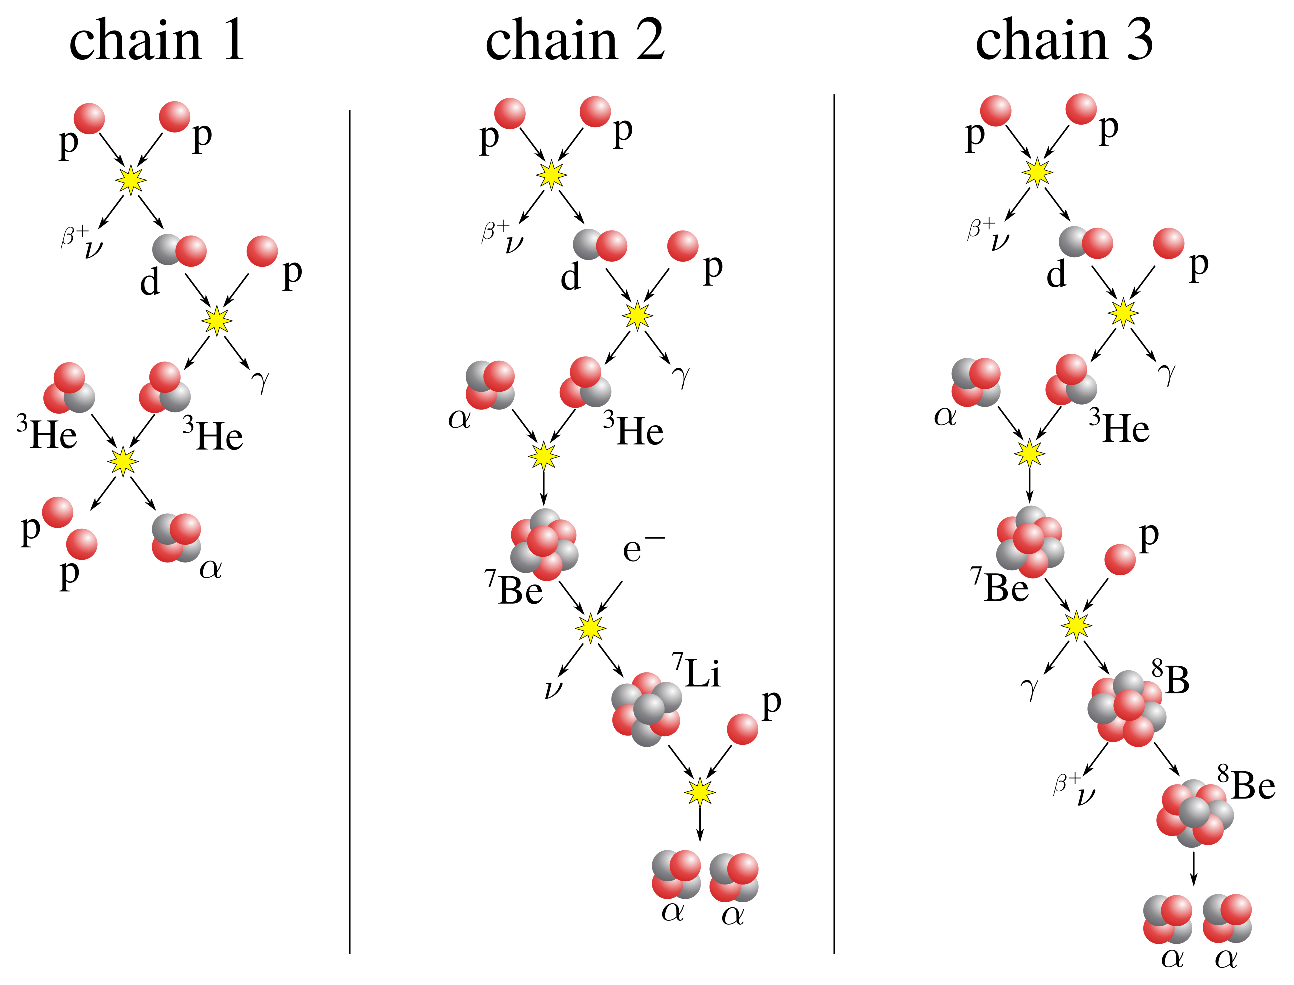
\includegraphics[clip, width=0.9\columnwidth]{pp_chain.eps}
  \caption{代表的なpp チェイン。pp チェインでは4つの陽子から1つの$\alpha$が生成される。}
  \label{fig::pp_chain}
\end{figure}

ppチェインにより$\alpha$が十分に生成された恒星では水素よりも重い$\alpha$が
より恒星の中心に集まり${\rm He}$コアを生成する。
${\rm He}$コアが重力により圧縮され温度がおよそ$10^8~{\rm K}$に達するとヘリウム燃焼が始まる。
${\rm He}$コアには十分な量の$\alpha$が存在するため、2つの$\alpha$が融合し${}^{8}{\rm Be}$が生成し、
崩壊するより早くもう1つ$\alpha$が融合して${}^{12}{\rm C}^{*}$になる。
このときに作られる${}^{12}{\rm C}$の多くはFred Hoyle が予言した$3\alpha$の
共鳴状態 (Hoyle状態、${\rm Ex} = 7.65{\rm MeV}$、$0_{2}^{+}$)~\cite{hoyle_state} となる。
Hoyle状態の${}^{12}{\rm C}$が$\gamma$線を放出し脱励起することで基底状態 (g.s.) になる (図\ref{fig::triple_alpha}左) 。
この3つの$\alpha$粒子が融合し${}^{12}{\rm C}$が生成される反応はトリプルアルファ反応と呼ばれる。
トリプルアルファ反応が恒星中で起こることでA = 4からA = 12へと直接移るため、A = 5, 8の壁を乗り越えることができる。
生成された${}^{12}{\rm C}$が更に$\alpha$を吸収することで${\rm O}$や${\rm Si}$などの更に重い核の合成へ進んでいく。
%\begin{equation}
%  \begin{array}{llll}
%%  \alpha(\alpha,\gamma){}^{8}{\rm Be}(\alpha,{}^{12}{\rm C}^{{\rm Hoyle}})
%%  \alpha(\alpha,\gamma){}^{8}{\rm Be}+\alpha\rightarrow{}^{12}{\rm C}^{{\rm Hoyle}}\label{eq::triplealpha}
%  %あとで矢印の絵を書こうかな
%    \alpha + \alpha \rightarrow & {}^{8}{\rm Be} & & \\
%    & {}^{8}{\rm Be} + \alpha \rightarrow & {}^{12}{\rm C}^{{\rm Hoyle}} &\\
%    & & {}^{12}{\rm C}^{{\rm Hoyle}} \rightarrow & {}^{12}{\rm C} + \gamma
%  \end{array}\label{eq::triplealpha}
%\end{equation}

\begin{figure}
  \centering
  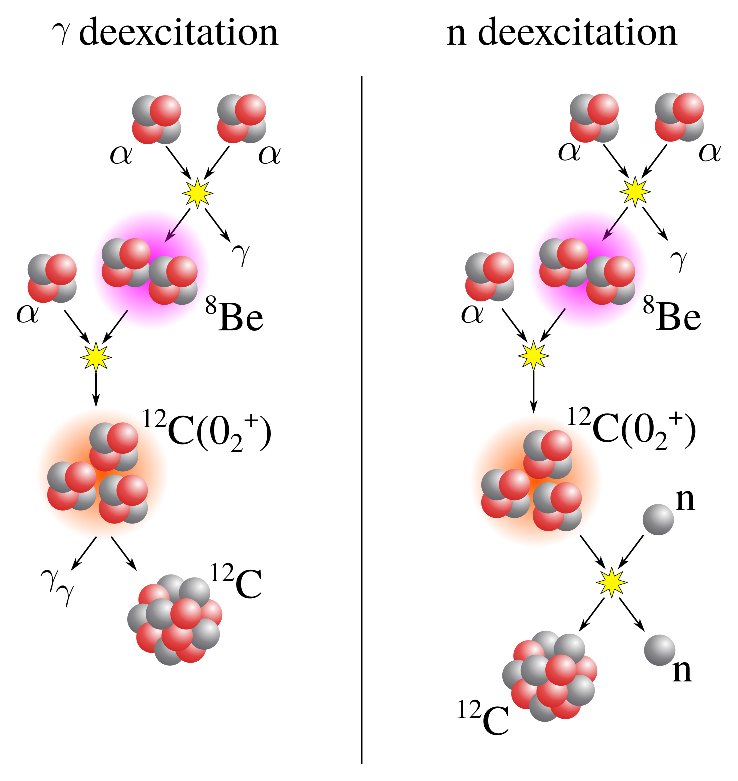
\includegraphics[clip, width=0.7\columnwidth]{triple_alpha.eps}
  %  \caption{トリプルアルファ反応。3つの$\alpha$粒子が反応し1つの${}^{12}{\rm C}$が生成される。}
  \caption[トリプルアルファ反応。]{トリプルアルファ反応。
    左は$\gamma$線を放出して脱励起するルート、右は中性子との散乱により脱励起するルートを表す。}
  \label{fig::triple_alpha}
\end{figure}

\section{高温高密度中でのトリプルアルファ反応}
\label{seq::triplealphareaction}
通常、トリプルアルファ反応で生成された$3\alpha$共鳴状態は図\ref{fig::triple_alpha} の左のように
$\gamma$線を放出することによって脱励起し、安定な${}^{12}{\rm C}$の基底状態になる。
近年、高温高密度領域では$\gamma$線による脱励起以外に、
図\ref{fig::triple_alpha} の右のように粒子との散乱による脱励起の
崩壊幅が増加することが示唆されている~\cite{hotdensemedium}。
これによりg.s.や$2_{1}^{+} ({\rm Ex} = 4.44 {\rm MeV}) $への脱励起が増加し、トリプルアルファ反応が加速されると考えられる。
粒子の中でも中性子は電荷を持っておらず、クーロン斥力を受けずに反応することができるため、
脱励起の増加への寄与が大きいと考えられる。

%\begin{equation}
%  \begin{array}{llll}
%    \alpha + \alpha \rightarrow & {}^{8}{\rm Be} & &\\
%    & {}^{8}{\rm Be} + \alpha \rightarrow & {}^{12}{\rm C}^{{\rm Hoyle}} &\\
%    & & {}^{12}{\rm C}^{{\rm Hoyle}} + {\rm X} \rightarrow & {}^{12}{\rm C} + {\rm X'}
%  \end{array}\label{eq::triplealpha_particle}
%\end{equation}

%\begin{figure}
%  \centering
%  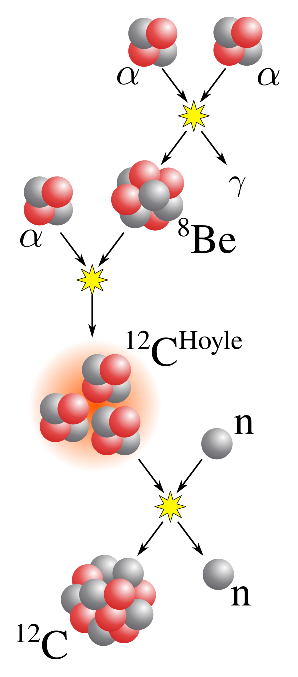
\includegraphics[clip, width=0.5\columnwidth]{triple_alpha_n.eps}
%  \caption[粒子との散乱により脱励起するトリプルアルファ反応。]{粒子との散乱により脱励起するトリプルアルファ反応。
%  この図では中性子と散乱する場合を表している。}
%  \label{fig::triple_alpha_n}
%\end{figure}

${}^{12}{\rm C}$と中性子の反応レートは
\begin{equation}
  r = N_{\rm n}N_{{}^{12}{\rm C}}\braket{\sigma v} {\rm cm}^{-3}{\rm s}^{-1}
  \label{eq::r}
\end{equation}
で与えられる。
ここで、$N_{{\rm n}}$は中性子の個数密度、
$N_{{}^{12}{\rm C}}$は${}^{12}{\rm C}$の個数密度を表す。
$\sigma$は中性子との散乱により始状態 (g.s.または$2_{1}^{+}$) からHoyle状態へ励起する全断面積であり、
$v$は中性子と${}^{12}{\rm C}$の相対速度である。
相対速度がMaxwell分布に従うとすると、${}^{12}{\rm C}({\rm n},{\rm n'}){}^{12}{\rm C}^{{\rm Hoyle}}$では
\begin{equation}
  \braket{\sigma v}_{\rm nn'} =
  \left(\frac{8}{\pi\mu}\right)^{1/2}\left(\frac{1}{kT}\right)^{^3/2}
  \int^{\infty}_{0}E'\sigma_{\rm n,n'}(E')\exp(-E'/kT)dE'
  \label{eq::sigmann'}
\end{equation}
となる。
$T$は温度、$\mu$は換算質量、$\sigma_{\rm n,n'}$は${}^{12}{\rm C}$の中性子非弾性散乱断面積である。
我々が考える反応は上記の逆過程 ${}^{12}{\rm C}^{{\rm Hoyle}}({\rm n',n}){}^{12}{\rm C}$ なので、
\begin{equation}
  \braket{\sigma v}_{\rm n'n} = \left(\frac{2I+1}{2I'+1}\right)
  \exp(-Q/kT)\braket{\sigma v}_{\rm nn'}
  \label{eq::sigman'n}
\end{equation}
となる。
ここで、$I$および$I'$は始状態 (g.s.または$2_{1}^{+}$)
および終状態 (Hoyle状態) のスピンである。
$Q$は$-7.65{\rm MeV}$ (g.s.の場合) または
$-3.21{\rm MeV}$ ($2_{1}^{+}$の場合) となる。
${}^{12}{\rm C}$ (Hoyle状態) の中性子非弾性散乱による脱励起の寿命は
\begin{equation}
  \tau_{\rm n'n}({}^{12}{\rm C}^{{\rm Hoyle}}) =
  (N_{\rm n}\braket{\sigma v}_{\rm n'n})^{-1} {\rm s}
  \label{eq::tau}
\end{equation}
となる。

中性子比弾性散乱による脱励起の寿命と$\gamma$線による脱励起の寿命 ($\tau_{\gamma} = 1.710\times10^{-13}~{\rm s}$) との比を
$R$とすると、
\begin{equation}
  R = 6.557\times10{-6}\times\rho_{\rm n}T_{9}^{-1.5}{\rm C}_{{\rm spin}}
  \int^{\infty}_{0}\sigma_{\rm nn'}(E)(E-Q)\exp(-11.605E/T_{9})dE
  \label{eq::R}
\end{equation}
と表される。
$E$はc.m.系のエネルギー、$\rho_{\rm n}$は中性子の質量密度 (${\rm g}/{\rm cm}^{3}$)、
$\sigma_{\rm nn'}(E')$は断面積 (${\rm mb}$)、$T_{9}$は温度 ($\times10^{9}~{\rm K}$) である。
${\rm C}_{{\rm spin}}$はg.s.からの場合1、
$2_{1}^{+}$からの場合5となる。
式(\ref{eq::R})からわかるように、中性子によって脱励起する過程は
特に温度に大きく依存する。
Beard らによる$R$と温度の依存性の計算結果~\cite{hotdensemedium}を図\ref{fig::R}に示す。
\begin{figure}
  \centering
  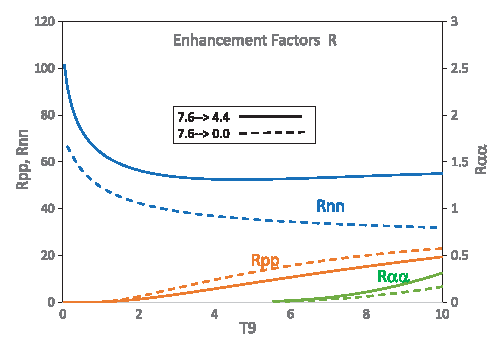
\includegraphics[clip, width=0.6\columnwidth]{R_T.eps}
  \caption[$\gamma$線による脱励起の寿命と粒子散乱による脱励起の寿命の比。]
          {$\gamma$線による脱励起の寿命と粒子散乱による脱励起の寿命の比~\cite{hotdensemedium}。
    Rnn、Rpp、R$\alpha\alpha$はそれぞれ中性子、陽子、$\alpha$粒子と散乱した際の寿命の比を表す。}
  \label{fig::R}
\end{figure}
図\ref{fig::R}は$\rho = 10^{6}~{\rm g}/{\rm cm}^{3}$の場合の結果を示している。
$\rho = 10^{6}~{\rm g}/{\rm cm}^{3}$という高密度下では$\gamma$線による脱励起に対して、
粒子による脱励起の寄与が大きくなることが分かる。
特に、中性子による寄与は$\gamma$線による寄与の40--100倍ととても大きい。

$\rho\sim10^{6}~{\rm g}/{\rm cm^{3}}, T\sim10^{9}~{\rm K}$のような高温高密度の環境は宇宙の何処にあるだろうか。
一つの候補として超新星爆発が考えられる。
10--30$\rm M_{\odot}$程度の大質量星は、重力崩壊を起こして星の一生を終える。
重力崩壊の際に恒星の中心にある鉄コアの温度が急激に上昇する。
極めて高い温度では高エネルギーの光子によって鉄コアの原子核が陽子や中性子に分解される (光分解反応)。
また、密度が非常に高いため式 (\ref{eq::neutronize}) のように陽子が中性子へ変わる電子捕獲が起きる。
\begin{equation}
  {\rm p}+{\rm e}^{-} \rightarrow {\rm p}+\nu_{\rm e}
  \label{eq::neutronize}
\end{equation}
すると、恒星の中心に原始中性子星が形成される。
重力によって中心に降ってくる物質は原始中性子星で跳ね返りが起こる。
この物質の跳ね返りが超新星爆発である。
崩壊前の恒星が持っていた重力エネルギーが熱エネルギーに変換されるので、
原始中性子星の表面温度は$10^10$~Kに達する。
跳ね返った物質が膨張することで温度が下がっていき、
$7\times10^9$~Kほどになると2つの陽子と2つの中性子が融合し$\alpha$粒子が生成される。
このとき、$\alpha$粒子と中性子が高密度かつ高温で存在する環境ができるのである。

\section{測定を行う中性子のエネルギー}
$R$を計算するためには、実験によって断面積 ($\sigma_{\rm nn'}$) のエネルギー分布が必要となる。
特に、天体中で${}^{12}{\rm C}$と散乱した後に中性子が持つエネルギー領域を狙う必要がある。
天体中の中性子の持つエネルギーはおよそ$k_{B}T$で表すことができる。
Beardら~\cite{hotdensemedium}が考えているような$T\sim10^{9}~{\rm K}$では、
中性子は$E_{\rm n'}\sim100~{\rm keV}$で運動している。% 1K = 8.61734e-5 eV
このような中性子がHoyle状態の${}^{12}{\rm C}$と散乱すると、
散乱後の中性子は$E_{\rm n}\sim8~{\rm MeV}$となる。
つまり、式 (\ref{eq::tau}) に示した脱励起の寿命の計算には
数〜十数 ${\rm MeV}$のエネルギーを持つ中性子と${}^{12}{\rm C}$との断面積のエネルギー分布が必要となる。
しかし、図\ref{fig::crosssection_pres}からも分かるように、数〜十数 ${\rm MeV}$の領域のデータがない。
そのため、このエネルギー領域での ${}^{12}{\rm C}({\rm n,n'}){}^{12}{\rm C}^{{\rm Hoyle}}$ の断面積の測定が必要である。
\begin{figure}
  \centering
  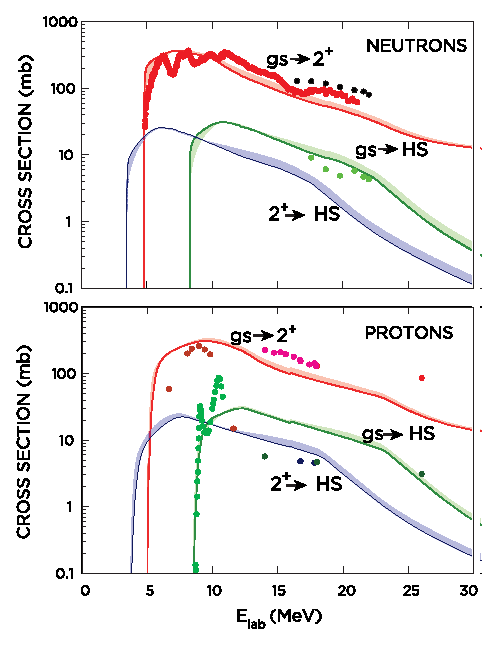
\includegraphics[clip,width=0.6\columnwidth]{cross_section_p_and_n.eps}
  \caption[${}^{12}{\rm C}$と中性子 (上段) および陽子 (下段) との非弾性散乱断面積。]
          {${}^{12}{\rm C}$と中性子 (上段) および陽子 (下段) との非弾性散乱断面積~\cite{hotdensemedium}。
  実線はTALYSを用いた理論計算、点は測定値を表す。}
  \label{fig::crosssection_pres}
\end{figure}

本研究ではその第一歩として$E_{\rm n} = 14~{\rm MeV}$の中性子を用いて断面積の測定を行う。
$14.1~{\rm MeV}$は式 (\ref{eq::dt}) に示すDT 反応で単色で生成可能なエネルギーである。
\begin{equation}
  {\rm d} + {\rm t} \rightarrow \alpha (3.5~{\rm MeV}) + {\rm n} (14~{\rm MeV})
  \label{eq::dt}
\end{equation}
このDT 反応で生成される$14~{\rm MeV}$の中性子と炭素との反応は核融合炉の開発で重要である。
ITERなどの核融合炉ではDT 反応を用いて質量エネルギーを取り出す。
核融合炉の中で生成される$14~{\rm MeV}$の中性子は構造材の原子核と反応し損傷させるため、
構造材の中に多く含まれる炭素との反応が詳しく調べられている。
そのため、すでに$14~{\rm MeV}$の中性子と${}^{12}{\rm C}$との断面積のデータがあり、本研究での測定結果との比較が可能となる。
単色エネルギーの中性子を生成可能であること、他データと測定結果の比較が可能であることの2点より、
測定方法の検証として$14~{\rm MeV}$の中性子で断面積の測定を行う。

$E_{\rm n}=14~{\rm MeV}$での${}^{12}{\rm C}({\rm n},{\rm n}'){}^{12}{\rm C}^{*}$の散乱断面積は
Ref.~\cite{takahashietal,kondoetal}によりすでに測定されている。
${}^{12}{\rm C}({\rm n},{\rm n}'+3\alpha)$反応の全断面積は209 mb、分岐比は表\ref{tab::branchingratio}となっている。
Ex = 7.65, 9.64, および10.3 MeVへ励起する反応が大部分を占めている。
微分断面積の角度分布は図\ref{fig::sig_angle_dist}のようである。
これらの測定値と比較することによって測定方法の妥当性を確認することが可能となる。

\begin{table}
  \centering
  \caption[${}^{12}{\rm C}(n,n'+3\alpha)$反応のチャンネルとその分岐比。]
          {${}^{12}{\rm C}(n,n'+3\alpha)$反応のチャンネルとその分岐比。
  ${}^{12}{\rm C}$の励起状態から$3\alpha$に、${}^{9}{\rm Be}$の励起状態から$2\alpha$に崩壊する。}
  \label{tab::branchingratio}
  \begin{tabular}{lc}
    \toprule
    \multicolumn{1}{c}{Reaction channel} & Branching ratio (\%)\\
    \midrule
    ${}^{12}{\rm C}({\rm n},{\rm n}'){}^{12}{\rm C}^{*}(7.65~{\rm MeV})$ & 4\\
    ${}^{12}{\rm C}({\rm n},{\rm n}'){}^{12}{\rm C}^{*}(9.64~{\rm MeV})$ & 33\\
    ${}^{12}{\rm C}({\rm n},{\rm n}'){}^{12}{\rm C}^{*}(10.3~{\rm MeV})$ & 16\\
    ${}^{12}{\rm C}({\rm n},{\rm n}'){}^{12}{\rm C}^{*}(10.84~{\rm MeV})$ & 6\\
    ${}^{12}{\rm C}({\rm n},{\rm n}'){}^{12}{\rm C}^{*}(11.83~{\rm MeV})$ & 4\\
    ${}^{12}{\rm C}({\rm n},\alpha){}^{9}{\rm Be}^{*}(1.68$--$3.05~{\rm MeV})$ & 24\\
    ${}^{12}{\rm C}({\rm n},\alpha){}^{9}{\rm Be}^{*}(4.7~{\rm MeV})$ & 13\\
    \bottomrule
  \end{tabular}
\end{table}

\begin{figure}
  \centering
  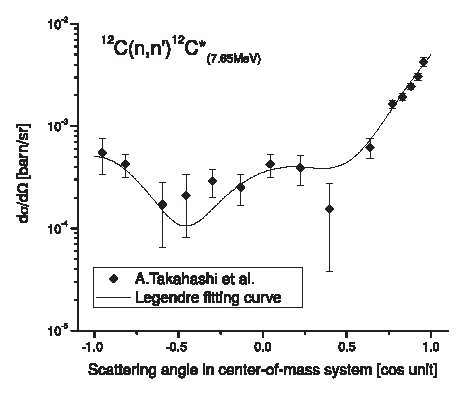
\includegraphics[clip, width=0.6\columnwidth]{cross_section_12C_n_n_12C_7.65.eps}
  \caption[${}^{12}{\rm C}({\rm n},{\rm n}'){}^{12}{\rm C}^{\rm Hoyle}$の微分断面積の角度分布。]
          {${}^{12}{\rm C}({\rm n},{\rm n}'){}^{12}{\rm C}^{\rm Hoyle}$の微分断面積の角度分布~\cite{kondoetal}。}
  \label{fig::sig_angle_dist}
\end{figure}

\section{大阪大学14 MeV 中性子工学実験装置 (OKTAVIAN)}
\begin{figure}
  \centering
  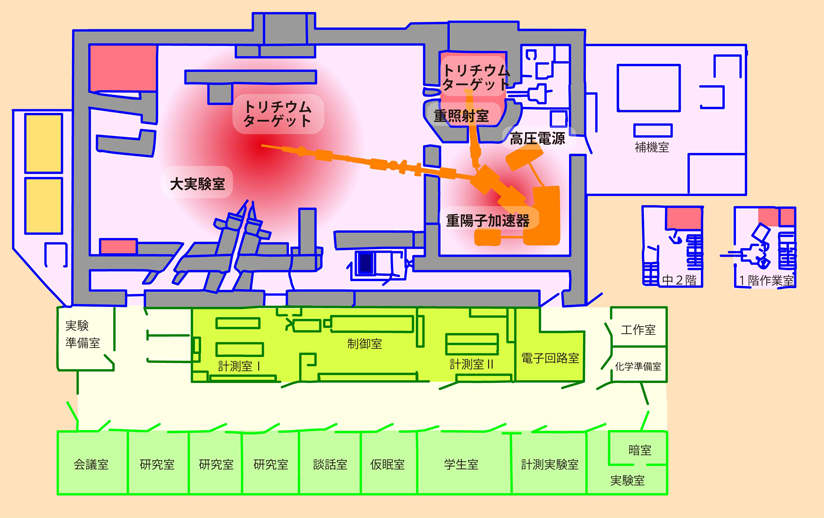
\includegraphics[clip, width=0.9\columnwidth]{oktavian-sketch.png}
  \caption[OKTAVIAN の施設図。]
          {OKTAVIAN の施設図。パルスビームラインとDC ビームラインがそれぞれ大実験室と重照射室に伸びている。}
  \label{pic::oktavian-sketch}
\end{figure}
大阪大学工学研究科のOKTAVIAN~\cite{oktavian} ではDT 反応により14 MeV の中性子を発生させることができる。
図\ref{pic::oktavian-sketch}にOKTAVIAN の施設図を示す。
OKTAVIAN は1981年から運転を開始し、核融合中性子工学研究に用いられてきた。
コッククロフト・ワルトン型加速器を用いて加速したデューテリウムをトリチウムターゲットに照射することで、
14 MeV の中性子を生成する。
OKTAVIAN にはパルスビームラインとDCビームラインの2つのビームラインがある。
パルスビームラインは大実験室に設置されたトリチウムターゲットを用いて、
DC ビームラインは重照射室に設置されたトリチウムターゲットを用いて中性子を生成する。

DC ビームラインで生成された中性子はトリチウムターゲットを中心に放射状に放出される。
この中性子を大実験室側へ取り出すための直径約100 mm の取り出し穴が重照射室と
大実験室を隔てる壁に空いている。
この取り出し穴から中性子を取り出すことで直径が約100 mmにコリメートされた
DC 中性子ビームを用いた測定を行うことができる。
ただし、DC ビームであるため中性子が入射した時間情報を得ることはできない。
パルスビームラインでは大実験室中にトリチウム標的が設置されているため、
中性子をコリメートすることができない。
その反面、パルス状に中性子が発生するので、中性子の時間情報を得ることができる。
本測定では、実験室内で反射した中性子によるバックグラウンドイベントを低減することや、
中性子の入射領域をコリメートできることから、DC ビームラインを用いる。

\section{測定に用いる実験装置}
\label{seq::detector_using_experiment}
本研究では${}^{12}{\rm C}^{\rm Hoyle}$から崩壊して生成した3つの$\alpha$粒子の直接測定を行う。
${}^{12}{\rm C}^{\rm Hoyle}$から放出された$\alpha$粒子は図\ref{fig::alpha_E_dist}のような分布を持つ。
図\ref{fig::alpha_E_dist}の塗りつぶしは全体の8割となる領域を示しており、
0--0.6 MeV である。
このような低エネルギーの$\alpha$粒子を効率よく検出するためには、
標的中で$\alpha$粒子が停止しないようにしなければならない。
例えば、$500~{\rm keV}$の$\alpha$粒子ではおよそ$350~{\rm \mu g/cm^2}$の炭素箔標的で停止してしまう。
標的中で止まってしまうような低エネルギー粒子の測定には、検出器が標的となるアクティブ標的が有効である。
図\ref{fig::alpha_theta_dist}は$\alpha$粒子の角度分布である。
図\ref{fig::alpha_theta_dist}の塗りつぶしは全体の8割となる領域を示しており、
0.13--1.31 rad. である。
%この図からもわかるように広い角度領域に$\alpha$粒子は崩壊する。
そのため、3つの$\alpha$粒子すべてを効率的に検出するためには大立体角を持つ検出器が必要となる。
このような要求を満たす検出器としてMAIKo TPC ($\mu$-PIC based active target for inverse kinematics .
time projection chamber)~\cite{maiko, mupic}がある。
MAIKo TPC はTPC の検出ガスを散乱標的として用い、
低エネルギーの荷電粒子を大立体角で検出するために開発された検出器である。
\begin{figure}
  \centering
  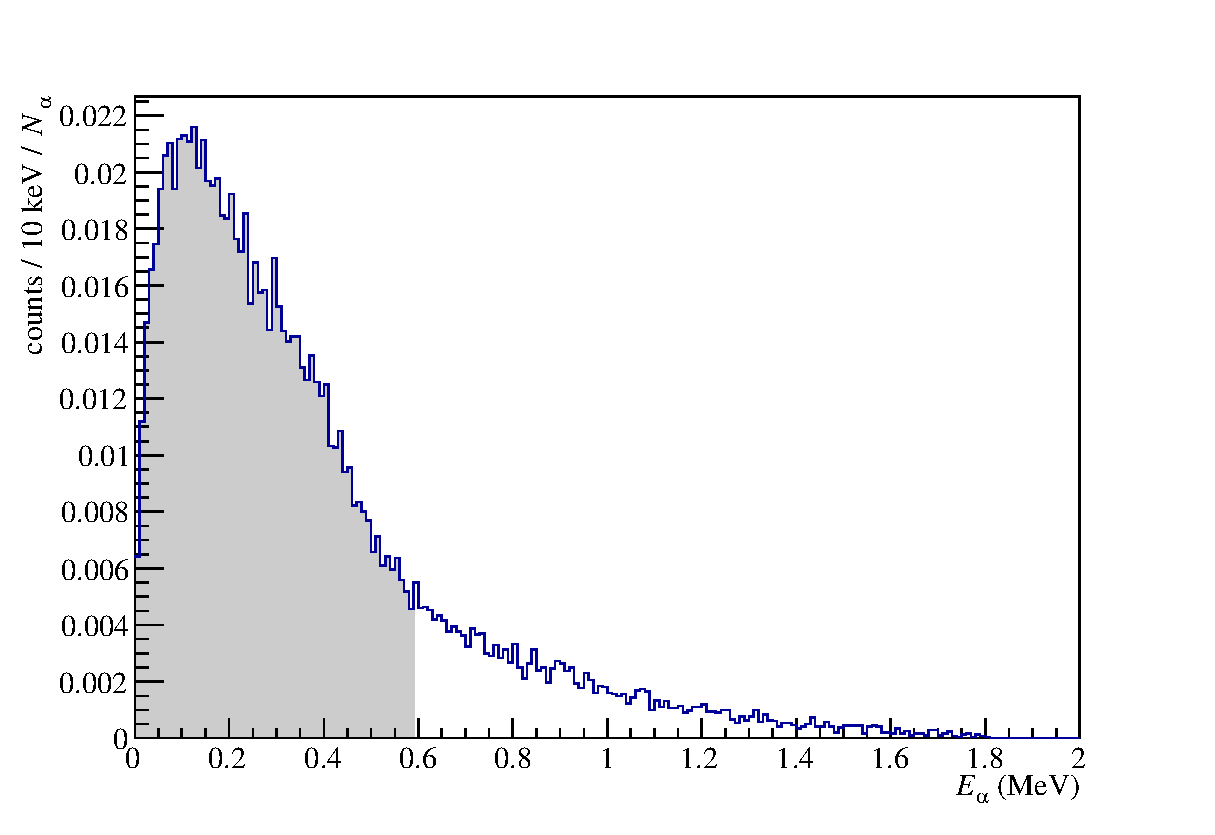
\includegraphics[clip, width=0.7\columnwidth]{alpha_e_dist_sim_region.eps}
  \caption[${}^{12}{\rm C}^{\rm Hoyle}$から放出された$\alpha$粒子のエネルギー分布。]
          {${}^{12}{\rm C}^{\rm Hoyle}$から放出された$\alpha$粒子のエネルギー分布。
            図は${}^{12}{\rm C}$から放出される3つの$\alpha$粒子すべての分布を表している。}
  \label{fig::alpha_E_dist}
  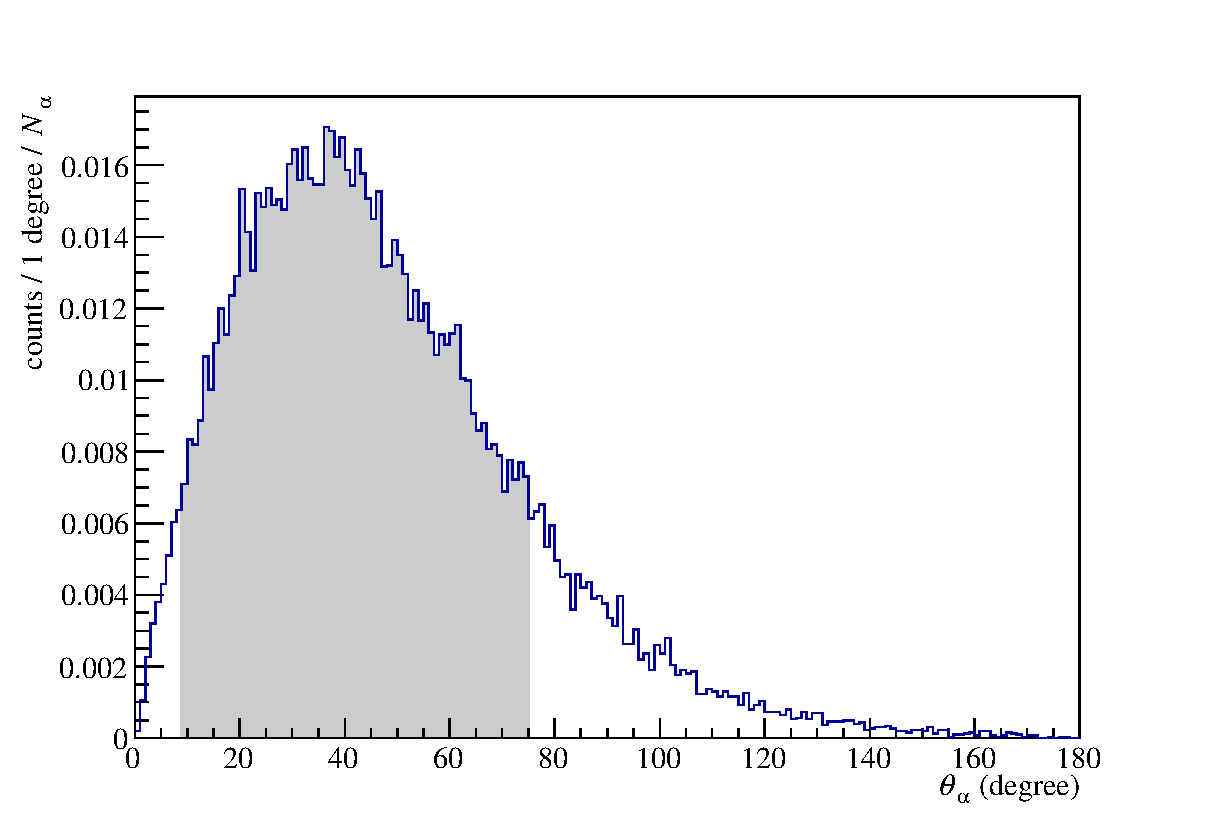
\includegraphics[clip, width=0.7\columnwidth]{alpha_theta_dist_region.eps}
  \caption[${}^{12}{\rm C}^{\rm Hoyle}$から放出された$\alpha$粒子の角度分布。]
          {${}^{12}{\rm C}^{\rm Hoyle}$から放出された$\alpha$粒子の角度分布。
            図は${}^{12}{\rm C}$から放出される3つの$\alpha$粒子すべての分布を表している。
          }
  \label{fig::alpha_theta_dist}
\end{figure}
MAIKo TPC を用いることで原理的には低エネルギーの$\alpha$粒子をほぼ4$\pi$で検出することができる。
本研究ではこれらの要求によりMAIKo TPC を用いて${}^{12}{\rm C}({\rm n},{\rm n}')3\alpha$反応を測定する。
%ピーク周りに8割を取ってくると0.13 rad -- 1.31 rad, 0 -- 0.595 MeV

%また、TPC は荷電粒子のトラックを検出することができる検出器である。
%荷電粒子を入射粒子として用いる実験では、標的粒子と散乱しなかった入射粒子のトラックも検出する。
%このような事象は背景事象となる。
%本研究では中性子を入射するため、そのような背景事象は発生しない。
%そのため、高強度の中性子ビームを用いた実験が可能であり、
%散乱事象を効率的に検出することができる。

\section{本研究の目的}
MAIKo TPC を用いた${}^{12}{\rm C}({\rm n},{\rm n}'){}^{12}{\rm C}^{\rm Hoyle}$の断面積測定のためには、
低エネルギーの$\alpha$粒子を検出する必要がある。
\ref{seq::detector_using_experiment}節で述べたように、
MAIKo TPC を用いることで効率的に3つの低エネルギー$\alpha$粒子を検出することが可能となる。
MAIKo TPC では使用する検出ガスの種類、圧力、電圧等の多くのパラメータを調整することができる。
本研究では効率よく$\alpha$粒子を検出することができる検出ガスの種類、圧力を検討した。
また、安定したにMAIKo TPC をオペレートする条件を検討した。

\end{document}
